% GNUPLOT: LaTeX picture with Postscript
\begingroup
  \makeatletter
  \providecommand\color[2][]{%
    \GenericError{(gnuplot) \space\space\space\@spaces}{%
      Package color not loaded in conjunction with
      terminal option `colourtext'%
    }{See the gnuplot documentation for explanation.%
    }{Either use 'blacktext' in gnuplot or load the package
      color.sty in LaTeX.}%
    \renewcommand\color[2][]{}%
  }%
  \providecommand\includegraphics[2][]{%
    \GenericError{(gnuplot) \space\space\space\@spaces}{%
      Package graphicx or graphics not loaded%
    }{See the gnuplot documentation for explanation.%
    }{The gnuplot epslatex terminal needs graphicx.sty or graphics.sty.}%
    \renewcommand\includegraphics[2][]{}%
  }%
  \providecommand\rotatebox[2]{#2}%
  \@ifundefined{ifGPcolor}{%
    \newif\ifGPcolor
    \GPcolorfalse
  }{}%
  \@ifundefined{ifGPblacktext}{%
    \newif\ifGPblacktext
    \GPblacktexttrue
  }{}%
  % define a \g@addto@macro without @ in the name:
  \let\gplgaddtomacro\g@addto@macro
  % define empty templates for all commands taking text:
  \gdef\gplbacktext{}%
  \gdef\gplfronttext{}%
  \makeatother
  \ifGPblacktext
    % no textcolor at all
    \def\colorrgb#1{}%
    \def\colorgray#1{}%
  \else
    % gray or color?
    \ifGPcolor
      \def\colorrgb#1{\color[rgb]{#1}}%
      \def\colorgray#1{\color[gray]{#1}}%
      \expandafter\def\csname LTw\endcsname{\color{white}}%
      \expandafter\def\csname LTb\endcsname{\color{black}}%
      \expandafter\def\csname LTa\endcsname{\color{black}}%
      \expandafter\def\csname LT0\endcsname{\color[rgb]{1,0,0}}%
      \expandafter\def\csname LT1\endcsname{\color[rgb]{0,1,0}}%
      \expandafter\def\csname LT2\endcsname{\color[rgb]{0,0,1}}%
      \expandafter\def\csname LT3\endcsname{\color[rgb]{1,0,1}}%
      \expandafter\def\csname LT4\endcsname{\color[rgb]{0,1,1}}%
      \expandafter\def\csname LT5\endcsname{\color[rgb]{1,1,0}}%
      \expandafter\def\csname LT6\endcsname{\color[rgb]{0,0,0}}%
      \expandafter\def\csname LT7\endcsname{\color[rgb]{1,0.3,0}}%
      \expandafter\def\csname LT8\endcsname{\color[rgb]{0.5,0.5,0.5}}%
    \else
      % gray
      \def\colorrgb#1{\color{black}}%
      \def\colorgray#1{\color[gray]{#1}}%
      \expandafter\def\csname LTw\endcsname{\color{white}}%
      \expandafter\def\csname LTb\endcsname{\color{black}}%
      \expandafter\def\csname LTa\endcsname{\color{black}}%
      \expandafter\def\csname LT0\endcsname{\color{black}}%
      \expandafter\def\csname LT1\endcsname{\color{black}}%
      \expandafter\def\csname LT2\endcsname{\color{black}}%
      \expandafter\def\csname LT3\endcsname{\color{black}}%
      \expandafter\def\csname LT4\endcsname{\color{black}}%
      \expandafter\def\csname LT5\endcsname{\color{black}}%
      \expandafter\def\csname LT6\endcsname{\color{black}}%
      \expandafter\def\csname LT7\endcsname{\color{black}}%
      \expandafter\def\csname LT8\endcsname{\color{black}}%
    \fi
  \fi
  \setlength{\unitlength}{0.0500bp}%
  \begin{picture}(9360.00,10080.00)%
    \gplgaddtomacro\gplbacktext{%
      \csname LTb\endcsname%
      \put(1210,704){\makebox(0,0)[r]{\strut{} 1100}}%
      \csname LTb\endcsname%
      \put(1210,1672){\makebox(0,0)[r]{\strut{} 1200}}%
      \csname LTb\endcsname%
      \put(1210,2640){\makebox(0,0)[r]{\strut{} 1300}}%
      \csname LTb\endcsname%
      \put(1210,3609){\makebox(0,0)[r]{\strut{} 1400}}%
      \csname LTb\endcsname%
      \put(1210,4577){\makebox(0,0)[r]{\strut{} 1500}}%
      \csname LTb\endcsname%
      \put(1210,5545){\makebox(0,0)[r]{\strut{} 1600}}%
      \csname LTb\endcsname%
      \put(1210,6513){\makebox(0,0)[r]{\strut{} 1700}}%
      \csname LTb\endcsname%
      \put(1210,7482){\makebox(0,0)[r]{\strut{} 1800}}%
      \csname LTb\endcsname%
      \put(1210,8450){\makebox(0,0)[r]{\strut{} 1900}}%
      \csname LTb\endcsname%
      \put(1210,9418){\makebox(0,0)[r]{\strut{} 2000}}%
      \csname LTb\endcsname%
      \put(1342,484){\makebox(0,0){\strut{} 80}}%
      \csname LTb\endcsname%
      \put(2069,484){\makebox(0,0){\strut{} 90}}%
      \csname LTb\endcsname%
      \put(2796,484){\makebox(0,0){\strut{} 100}}%
      \csname LTb\endcsname%
      \put(3523,484){\makebox(0,0){\strut{} 110}}%
      \csname LTb\endcsname%
      \put(4250,484){\makebox(0,0){\strut{} 120}}%
      \csname LTb\endcsname%
      \put(4976,484){\makebox(0,0){\strut{} 130}}%
      \csname LTb\endcsname%
      \put(5703,484){\makebox(0,0){\strut{} 140}}%
      \csname LTb\endcsname%
      \put(6430,484){\makebox(0,0){\strut{} 150}}%
      \csname LTb\endcsname%
      \put(7157,484){\makebox(0,0){\strut{} 160}}%
      \csname LTb\endcsname%
      \put(7884,484){\makebox(0,0){\strut{} 170}}%
      \put(8016,704){\makebox(0,0)[l]{\strut{} 1100}}%
      \put(8016,1672){\makebox(0,0)[l]{\strut{} 1200}}%
      \put(8016,2640){\makebox(0,0)[l]{\strut{} 1300}}%
      \put(8016,3609){\makebox(0,0)[l]{\strut{} 1400}}%
      \put(8016,4577){\makebox(0,0)[l]{\strut{} 1500}}%
      \put(8016,5545){\makebox(0,0)[l]{\strut{} 1600}}%
      \put(8016,6513){\makebox(0,0)[l]{\strut{} 1700}}%
      \put(8016,7482){\makebox(0,0)[l]{\strut{} 1800}}%
      \put(8016,8450){\makebox(0,0)[l]{\strut{} 1900}}%
      \put(8016,9418){\makebox(0,0)[l]{\strut{} 2000}}%
      \put(1342,9638){\makebox(0,0){\strut{} 80}}%
      \put(2069,9638){\makebox(0,0){\strut{} 90}}%
      \put(2796,9638){\makebox(0,0){\strut{} 100}}%
      \put(3523,9638){\makebox(0,0){\strut{} 110}}%
      \put(4250,9638){\makebox(0,0){\strut{} 120}}%
      \put(4976,9638){\makebox(0,0){\strut{} 130}}%
      \put(5703,9638){\makebox(0,0){\strut{} 140}}%
      \put(6430,9638){\makebox(0,0){\strut{} 150}}%
      \put(7157,9638){\makebox(0,0){\strut{} 160}}%
      \put(7884,9638){\makebox(0,0){\strut{} 170}}%
      \put(308,5061){\rotatebox{-270}{\makebox(0,0){\strut{}Weight (lb)}}}%
      \put(8917,5061){\rotatebox{-270}{\makebox(0,0){\strut{}Weight (lb)}}}%
      \put(4613,154){\makebox(0,0){\strut{}Moment/1000 (pound-inches)}}%
      \put(4613,9967){\makebox(0,0){\strut{}Moment/1000 (pound-inches)}}%
    }%
    \gplgaddtomacro\gplfronttext{%
      \put(3523,8934){\makebox(0,0){\strut{}\Large \bfseries \sffamily Normal Weight/Moment Envelope}}%
      \put(3159,7240){\makebox(0,0){\strut{}\Large \bfseries \sffamily Restricted Aerobatic}}%
      \put(3159,6755){\makebox(0,0){\strut{}\Large \bfseries \sffamily Weight/Moment Envelope}}%
      \put(5340,1188){\makebox(0,0){\strut{}\Large \bfseries \sffamily Aerobatic Weight/Moment Envelope}}%
    }%
    \gplbacktext
    \put(0,0){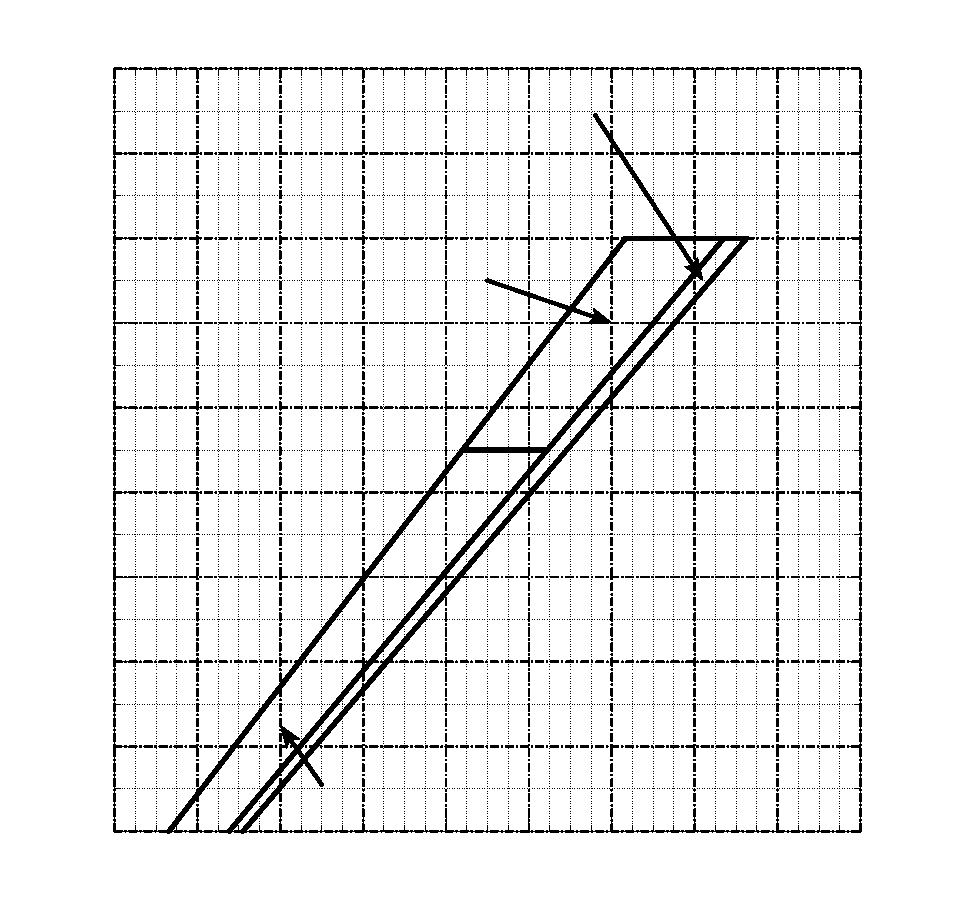
\includegraphics{../graphs/wb-moment-chart1800}}%
    \gplfronttext
  \end{picture}%
\endgroup
